%%% Template originaly created by Karol Kozioł (mail@karol-koziol.net) and modified for ShareLaTeX use

\documentclass[a4paper,11pt]{article}

\usepackage[T1]{fontenc}
\usepackage[utf8]{inputenc}
\usepackage{graphicx}
\usepackage{xcolor}

\renewcommand\familydefault{\sfdefault}
\usepackage{tgheros}

\usepackage{amsmath,amssymb,amsthm,textcomp}
\usepackage{enumerate}
\usepackage{multicol}
\usepackage{tikz}

\usepackage{geometry}
\geometry{left=25mm,right=25mm,%
bindingoffset=0mm, top=20mm,bottom=20mm}

\usepackage[export]{adjustbox}
\usepackage{subcaption}
\usepackage{float}

\usepackage{amsmath}
\usepackage{amssymb}
\usepackage{amsthm}


\linespread{1.3}

\newcommand{\linia}{\rule{\linewidth}{0.5pt}}

% custom theorems if needed
\newtheoremstyle{mytheor}
 {1ex}{1ex}{\normalfont}{0pt}{\scshape}{.}{1ex}
 {{\thmname{#1 }}{\thmnumber{#2}}{\thmnote{ (#3)}}}

\theoremstyle{mytheor}
\newtheorem{defi}{Definition}

% my own titles
\makeatletter
\renewcommand{\maketitle}{
\begin{center}
\vspace{2ex}
{\huge \textsc{\@title}}
\vspace{1ex}
\\
\linia\\
\@author \hfill \@date
\vspace{4ex}
\end{center}
}
\makeatother
%%%

% custom footers and headers
\usepackage{fancyhdr}
\pagestyle{fancy}
\lhead{}
\chead{}
\rhead{}
\lfoot{Kryptografia, Lista 2}
\cfoot{}
\rfoot{Page \thepage}
\renewcommand{\headrulewidth}{0pt}
\renewcommand{\footrulewidth}{0pt}
%

%%%----------%%%----------%%%----------%%%----------%%%

\begin{document}

\title{Kryptografia, Lista 2}

\author{Adrian Mucha, Politechnika Wrocławska, WPPT}

\date{17/05/2020}

\maketitle

\section*{AES vs. DES}
% Please add the following required packages to your document preamble:
% \usepackage{graphicx}
\begin{table}[H]
    \begin{tabular}{|p{0.5\textwidth}|p{0.5\textwidth}|}
        \hline
        \multicolumn{1}{|c|}{\textbf{AES}}                                                 & \multicolumn{1}{c|}{\textbf{DES}}                                                                         \\ \hline
        AES: Advanced Encryption Standard                                                  & DES: Data Encryption Standard                                                                             \\ \hline
        Klucze mają długość 128, 192 lub 256 bitów                                         & Długość klucza to 56 bitów.                                                                               \\ \hline
        Liczba rund w zależności od klucza: 10(128-bitów), 12(192-bitów) lub 14(256-bitów) & 16 rund identycznych operacji                                                                             \\ \hline
        Struktura opiera się o sieć substytucyjno-permutacyjną.                            & Struktura opiera się o sieci Feistela.                                                                    \\ \hline
        AES jest bezpieczniejszy niż DES i jest światowym standardem.                      & DES może być łatwo złamany i ma wiele znanych słabości. Istnieje 3DES który jest bezpieczniejszy niż DES. \\ \hline
        Koduje 128 bitów tekstu jawnego.                                                   & Koduje 64 bity tekstu jawnego.                                                                            \\ \hline
        Brak znanych ataków crypto-analitycznych prócz ataków side channel.                & Znane ataki: Brute-force, Linear crypt-analysis oraz Differential crypt-analysis.                         \\ \hline
    \end{tabular}
    \label{tab:my-table}
\end{table}

\section*{Tryby AES}
AES obsługuje różne tryby operowania na danych, które posiadają różne właściwości i stopnie bezpieczeństwa oraz szybkości działania czy możliwości pracy równoległej na wielu blokach. Tabela \ref{tab:aesmodes} przedstawia zalety i wady różnych trybów operowania.

\subsection*{Słabość w trybie ECB}
Przykład słabości szyfrowania w trybie ECB. Gołym okiem widać powtarzające się szyfrogramy oraz wzorce na obrazku \ref{fig:compare}.

\begin{figure}[]
    \begin{subfigure}{0.33\textwidth}
        
\includegraphics[width=1.0\linewidth]{logo_original.png}
        \caption{Zdjęcie oryginalne}
        \label{fig:original}
    \end{subfigure}
    \begin{subfigure}{0.33\textwidth}
        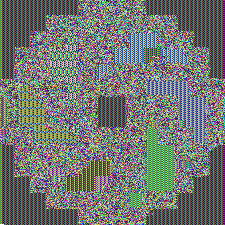
\includegraphics[width=1.0\linewidth]{logo_des_ecb.png}
        \caption{ECB}
        \label{fig:ecb}
    \end{subfigure}
    \begin{subfigure}{0.33\textwidth}
        
\includegraphics[width=1.0\linewidth]{logo_des_cbc.png}
        \caption{CBC}
        \label{fig:cbc}
    \end{subfigure}

    \caption{Obrazy przedstawiają różnice w kodowaniu przykładowego obrazu za pomocą ECB oraz CBC. Można zauważyć, że tryb ECB zawiera powtórzenia w szyfrogramach jeżeli w tekście jawnym również takowe się znajdują.}
    \label{fig:compare}
\end{figure}

\subsection*{Bezpieczeństwo CBC}
Tryb CBC jest wystawiony na \textit{atak z wybranym tekstem jawnym} jeżeli wektor inicjalizujący \texttt{IV} nie będzie wybierany losowo przez nadawcę. Jeżeli adwersarz potrafi przewidzieć \texttt{IV} to będzie mógł zastosować wyżej wymieniony atak. Atak przedstawia obrazek \ref{fig:cpa}.

\begin{figure}[]
    \begin{subfigure}{\textwidth}
        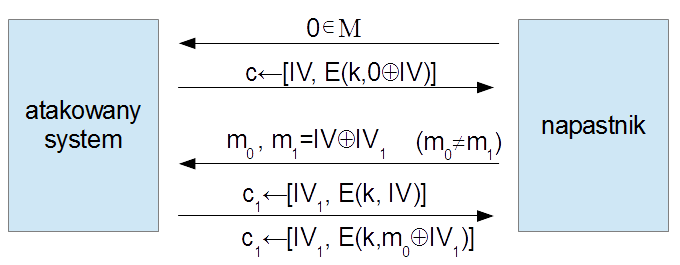
\includegraphics[width=1.0\linewidth]{cbc_atak_cpa.png}
    \end{subfigure}

    \caption{Atak z wybranym tekstem jawnym (CPA) na tryb szyfrowania CBC.}
    \label{fig:cpa}
\end{figure}

\begin{table}[]
    \begin{tabular}{|p{0.1\textwidth}|p{0.45\textwidth}|p{0.45\textwidth}|}
        \hline
        \multicolumn{1}{|c}{\textbf{Tryb}} & \multicolumn{1}{|c|}{\textbf{Zalety}} & \multicolumn{1}{|c|}{\textbf{Wady}}
        \\ \hline
        ECB & \begin{itemize}
            \setlength\itemsep{-0.5em}
            \item Prosty
            \item Szybki
            \item Równoległy
        \end{itemize} & \begin{itemize}
            \setlength\itemsep{-0.8em}
            \item Powtórzenia tekstu jawnego będą widoczne w szyfrze
            \item Uszkodzony szyfr będzie mieć wpływ na tekst jawny
            \item Brak odporności na \textit{replay attacks}
            \item Nie powinno się go używać
        \end{itemize}
        \\ \hline

        CBC & \begin{itemize}
            \setlength\itemsep{-0.5em}
            \item Równoległe odszyfrowywanie
            \item Powtórzenia nie będą widoczne w szyfrze
        \end{itemize} & \begin{itemize}
            \setlength\itemsep{-0.8em}
            \item Brak równoległego szyfrowania
            \item Uszkodzony blok wpływa na kolejne bloki
        \end{itemize}
        \\ \hline

        CFB & \begin{itemize}
            \setlength\itemsep{-0.5em}
            \item Brak wyrównania (no padding)
            \item Równoległe odszyfrowywanie
        \end{itemize} & \begin{itemize}
            \setlength\itemsep{-0.8em}
            \item Brak równoległego szyfrowania
            \item Brak odporności na \textit{replay attack}
            \item Uszkodzony blok wpływa na kolejne bloki
        \end{itemize}
        \\ \hline

        OFB & \begin{itemize}
            \setlength\itemsep{-0.5em}
            \item Brak wyrównania (no padding)
            \item Szyfrowanie i deszyfrowanie używa tego samego schematu
            \item Uszkodzony blok nie wpływa na inne
        \end{itemize} & \begin{itemize}
            \setlength\itemsep{-0.8em}
            \item Brak równoległego szyfrowania
            \item Adwersarz może zmienić uszkodzić część szyfru by zmienić tekst jawny
        \end{itemize}
        \\ \hline
        
        CTR & \begin{itemize}
            \setlength\itemsep{-0.5em}
            \item Brak wyrównania (no padding)
            \item Równoległe szyfrowanie i deszyfrowanie
            \item Szyfrowanie i deszyfrowanie używa tego samego schematu
            \item Uszkodzony blok nie wpływa na inne
        \end{itemize} & \begin{itemize}
            \setlength\itemsep{-0.8em}
            \item Adwersarz może zmienić uszkodzić część szyfru by zmienić tekst jawny
        \end{itemize}
        \\ \hline
    \end{tabular}
    \caption{Wady i zalety różnych trybów AES.}
    \label{tab:aesmodes}
\end{table}

\section*{Zad 1 \& 2}
\subsection*{Program szyfrujący/deszyfrujący oraz keystore}
Program \texttt{index.ts} korzysta z mechanizmów szyfrujących dostarczanych przez \texttt{OpenSSL}. W szczególności używa dostępnych trybów \texttt{AES} (\texttt{CBC, OFB, CTR}) o długości klucza $256$ bitów. Do celów demonstracyjnych \texttt{IV} jest stałe ($0...0$) - nie powinno się tak robić.

Pliki są przetwarzane strumieniowo dzięki czemu możemy przetwarzać dane dowolnej wielkości bez potrzeby ładowania całości do pamięci. Przed szyfrowaniem pliki są dodatkowo kompresowane za pomocą \texttt{Gzip}. Zaletą programu jest to, że operuje na plikach tymczasowych i na końcu zastępuje szyfrowany plik, przez co unikamy możliwości uszkodzenia oryginalnego pliku gdyby wystąpił błąd podczas pracy programu i całość podmieniana jest już z gotowym zaszyfrowanym plikiem.

Program używa biblioteki opensource \texttt{key-store} do obsługi keystore'a i przechowuje klucze w pliku \texttt{store.jsks}. Plik \texttt{store.ts} jest odpowiedzialny za odczyt/zapis keystore'a. Nowe klucze można dodawać za pomocą skryptu \texttt{newKey.ts}.

Program obsługuje argumenty linii komend, które można wyświetlić za pomocą \texttt{----help}.

\subsubsection*{Uruchamianie}
Wymagane środowisko \texttt{Node.js} w wersji \texttt{10 >=}.
\begin{enumerate}
    \item \texttt{npm install} - instaluje zależności
    \item \texttt{npm run encrypt ---- [lista argumentów]}
\end{enumerate}

\subsection*{Oracle \& challenge}
Plik \texttt{oracle.ts} można uruchomić jako serwer nasłuchujący na porcie $3000$ na zapytania typu \texttt{POST}, który jako odpowiedź zwraca zaszyfrowane wiadomości. \texttt{IV} jest celowo zwiększane o $1$ z każdą zaszyfrowaną wiadomością.

Skrypt \texttt{zad2.ts} jest atakiem CPA wykorzystującym \textit{,,lukę w systemie"} dzięki której jest w stanie przewidywać następne \texttt{IV} i z powodzeniem rozróżnić wiadomości zakodowane w challenge'u. Atak został przedstawiony na schemacie \ref{fig:cpa}.

\subsubsection*{Uruchamianie}
Wymagane środowisko \texttt{Node.js} w wersji \texttt{10 >=}.
\begin{enumerate}
    \item \texttt{npm install} - instaluje zależności
    \item \texttt{npm start} - uruchamia wyrocznię oraz challenge
    \item \texttt{npm run crack} - uruchamia skrypt wygrywający atak CPA na \texttt{AES-256-CBC} gdy \texttt{IV} jest przewidywalne
\end{enumerate}

\end{document}